\documentclass[a4paper,10pt]{article}

\usepackage{microtype}
\usepackage{pdfpages}
\usepackage{graphicx}
\usepackage{keyval}
  \setkeys{Gin}{width=\textwidth, keepaspectratio}
\usepackage{amsmath}
\usepackage[margin=2.5cm]{geometry}
\usepackage{lscape}
%\usepackage{setspace}
%  \doublespacing
%\usepackage{enumitem}
%  \setlist{nolistsep}
\usepackage{booktabs}
\usepackage{dcolumn}
  \newcolumntype{d}{D{.}{.}{5.1}}
\usepackage[utopia]{mathdesign}

\renewcommand{\deg}{$^\circ$}
\setlength{\parindent}{0pt}
\setlength{\parskip}{2ex}


\title{CE5703 Assignment 2---Jacket Lifting Analysis}
       
\author{Mohanadas Harish Chandar \\
        U067314J}

\date{November 23, 2009}

\begin{document}
\maketitle

\section*{Introduction}
Analysis of an offshore jacket lifing process was carried out. 
The jacket was to be lifted off the transport barge and subsequently upended 
using sequential manipulation of the crane barge's 2 selected hooks.
The design guide used was the McDermott in-house guide.

\section*{Crane barge}
The crane barge chosen was Asian Hurcules II. 
The barge stern is assumed to be 20\,m from the quayside and a 
jib offset of 20\deg\ is chosen. 
Thus, horizontal distance between main hook and jib hook 
$= 48 - 22 = 26\,\mathrm{m}$.

The lift capacity charts show that the crane barge has sufficient capacity 
and clearance for the lifting operation. 

\section{Sling tensions and appropriate slings compatible with rigging system}
Since the jacket was not weighed, a weight contingency factor (CF) of 1.1 is 
applied to the calculated weight (W).
\begin{align*}
\text{Gross weight} &= \mathrm{W} \times \mathrm{CF} \\
                    &= 450\,\mathrm{t} \times 1.1 \\
                    &= 495\,\mathrm{t}
\end{align*}

Since lift is being conducted offshore by a single vessel, a dynamic 
amplification factor (DAF) of 1.2 is applied.
\begin{align*}
\text{Lift weight} &= \text{gross weight} \times \mathrm{DAF} \\
                   &= 496\,\mathrm{t} \times 1.2 \\
                   &= 594\,\mathrm{t}
\end{align*}

Rigging weight is assumed to be 6\,t. Thus,
\begin{align*}
\text{Hook load} &= \text{lift weight} + \text{rigging weight} \\
                 &= 594\,\mathrm{t} + 6\,\mathrm{t} \\
                 &= 600\,\mathrm{t}
\end{align*}

\subsection*{Sling tensions at lift off}
Considering equilibrium and taking moments about point A:
\begin{align}
H_1 \cos{\phi_1} &= H_2 \cos{\phi_2} \\
H_1 \sin{\phi_1} + H_2 \sin{\phi_2} &= 600\,\mathrm{t}
\end{align}
\begin{align}
H_2 \sin{\phi_2} (30) &= 600 (16) \\ \nonumber
H_2 \sin{\phi_2} &= 320\,\mathrm{t}
\end{align}
\begin{align*}
H_1 \sin{\phi_1} &= 600 - 320 = 280\,\mathrm{t}
\end{align*}

Consider the case of $\phi_1$ = 75\deg\,

From Eqn 1, 
\begin{align*}
H_2 \cos{\phi_2} &= \frac{280}{\sin{75^\circ}} \times \cos{75^\circ} 
                  = 75\,\mathrm{t}
\end{align*}

Combining with Eqn 3,
\begin{align*}
\tan{\phi_2} &= \frac{320}{75} = 4.27 \\
\phi_2 &= 76.8^\circ
\end{align*}

\begin{align*}
H_1 &= \frac{280}{\sin{75^\circ}} = 290\,\mathrm{t} \\
H_2 &= \frac{75}{\cos{76.8^\circ}} = 328\,\mathrm{t}
\end{align*}

For preliminary calculations, assume sling angles 
$\phi_1$ and $\phi_2$ = 70\deg. 

Thus, sling tensions
\begin{align*}
T_1 \text{ at A} &= \frac{H_1}{2 \cos{20^\circ}} = 154\,\mathrm{t} \\
T_2 \text{ at B} &= \frac{H_2}{2 \cos{20^\circ}} = 175\,\mathrm{t} \\
\end{align*}

\subsection*{Sling tensions when jacket is vertical}
Distance between diagonally opposite lift points 
$= \sqrt{14.15^2 +19.15^2} = 23.81\,\mathrm{m}$.
Thus, minimum sling length to achieve $>60^\circ$ angle to the 
horizontal is 24\,m.

Since lifting arrangement is indeterminate, a skew factor of 1.5 
(75-25) is applied.

\begin{align*}
\text{Factored hook load} &= 1.5 \times 600 = 750\,\mathrm{t}
\end{align*}

Consider an angle of 30\deg\ between the slings and the vertical:

\begin{align*}
T_1 &= \frac{750}{4 \cos{30^\circ}} = 217\,\mathrm{t}
\end{align*}



\subsection*{Sling selection}
Considering fairly calm conditions during installation, a factor of safety of
3 is taken for sling selection.

For $T_1$, required MBL = $217 \times 3 = 651\,\mathrm{t}$ \\
For $T_2$, required MBL = $175 \times 3 = 525\,\mathrm{t}$

From Asian Lift slings list, \\
Use slings $\Phi 103\,\mathrm{mm} \times 27.5\,\mathrm{m}$ length for 
$T_1$, MBL = 800\,t. \\
Use slings $\Phi 90\,\mathrm{mm} \times 13\,\mathrm{m}$ length for 
$T_2$, MBL = 556\,t.

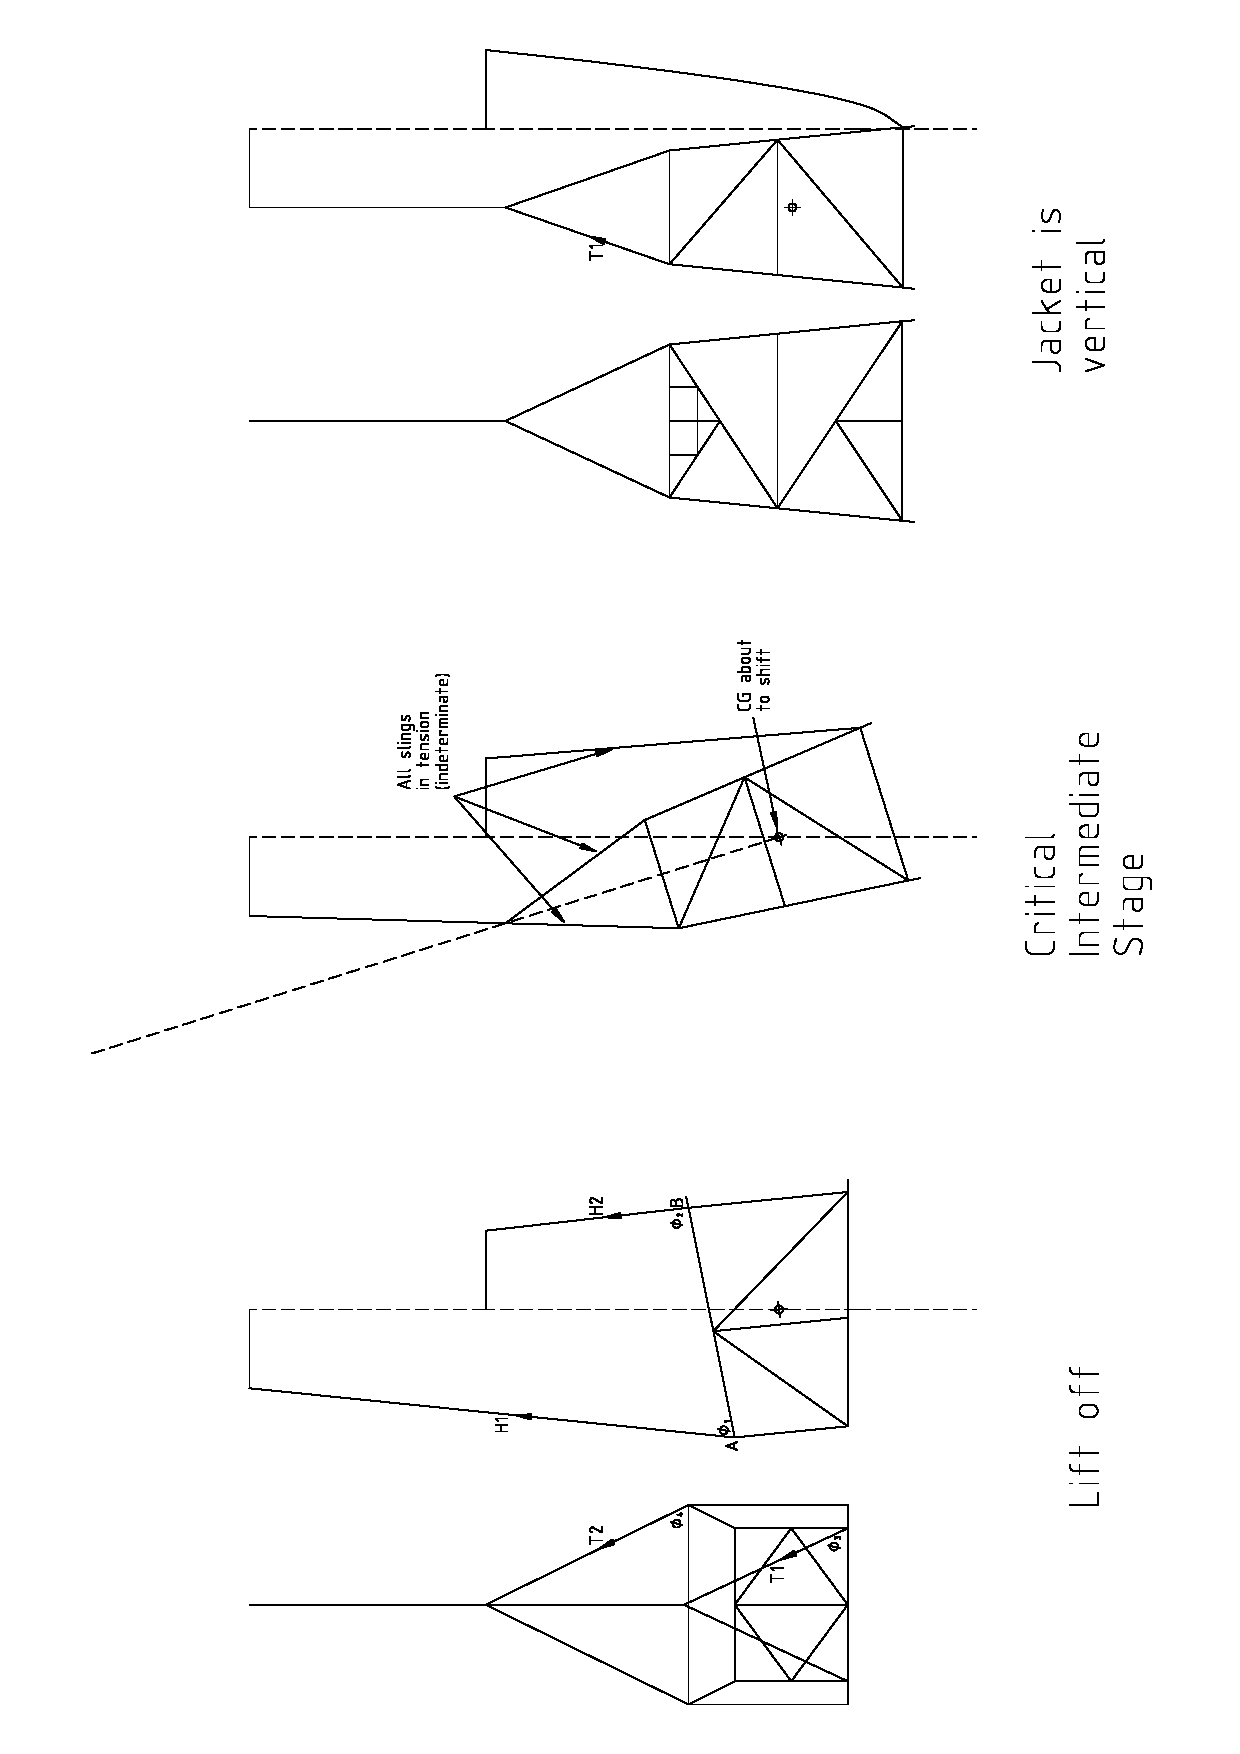
\includepdf[landscape, angle=-90]{visualisation}

\addtocounter{section}{1}
\section{Trunnion and padeye design}
\subsection*{Trunnions for bottom framing}
To adopt a factor of safety consistent with the other rigging components
(slings, etc.), a safety factor of 2 is adopted.

Required trunnion brace strength $> 2 \times 175\,\mathrm{t} = 350\,\mathrm{t}$.

Consider brace/sling diameter ratio of 4 to ensure bending loss in sling is 
minimised), \\
brace diameter $> 4 \times 90\,\mathrm{mm} = 360\,\mathrm{mm}$. 

End plate diameter $> \text{trunnion brace dismeter} + 1.2 \times 
                      \text{sling diameter}$

Shear strength of brace $= \frac{A_v \sigma_y}{\sqrt{3}} 
                         = \frac{2 d t \sigma_y}{\sqrt{3}}$.

{\bf Choose brace with $d$ = 500\,mm and $t$ = 20\,mm;} \\
Brace strength $= \frac{2 \times 500 \times 20 \times 345}{\sqrt{3}} \mathrm{N}
                = 3980\,\mathrm{kN}
                = 398\,\mathrm{t}$ (OK)

{\bf Choose end plate with $d$ = 610\,mm and $t$ = 20\,mm;} \\
End plate diameter $> 500\,\mathrm{mm} + 1.2 \times 90\,\mathrm{mm}
                    = 608\,\mathrm{mm}$ (OK)

{\bf Choose bearing plate with $d$ = 460\,mm and $t$ = 25\,mm;} \\
Bearing stress is taken as 0.9$f_y$. \\
Bearing plate thickness $> \frac{350 \times 10 \times 1000}
                                 {500 \times 345 \times 0.9} \mathrm{mm}
                         = 22.5\,\mathrm{mm}$ (OK)

\subsection*{Padeyes for top framing}
To adopt a factor of safety consistent with the other rigging components
(slings, etc.), a safety factor of 2 is adopted.

Required shackle safe working load, $P > 2 \times 217\,\mathrm{t} = 434\,\mathrm{t}$.

From Asian Lift shackles list, \\
Use SWL 500\,t Crosby W/Body Shackle, pin $\Phi$ 181\,mm, 
inside width 250\,mm, inside length $\Phi$ 666\,mm.

Taking $d$ as pin diameter, and $W$ as pin inside length, \\
Diameter of lifting eye hole, $D = d \times 1.04 = 181 \times 1.04 
                                 = 188\,\mathrm{mm}$.

{\bf Choose Use main plate, $T$ = 104\,mm, $R$ = 226\,mm, and 
cheek plate, $t$ = 64\,mm, $r$ = 200\,mm;}

Edge distance, $R \ge 1.25 D = 1.25 \times 181 = 226\,\mathrm{mm}$ (OK)

Combined thickness of main plate and cheek plates, 
$a \approx W - 12\,\mathrm{mm} = 250 - 12 = 238\,\mathrm{mm}$ \\
$a = 104 + 2 \times 64 = 232\,\mathrm{mm}$ (OK)

Bearing stress, 
$f_p = \frac{P}{Da} = \frac{434 \times 10000}{188 \times 232}\,\mathrm{MPa}
                    = 99.5\,\mathrm{MPa} < 0.9f_y = 270\,\mathrm{MPa}$ (OK)

Pull-out shear stress,
$f_{ps} = \frac{P/2}{2t(r-0.5D) + T(R-0.5D)}
        = \frac{434 \times 10000 / 2}
               {2 \times 64(200-0.5\times188) + 104(226-0.5\times188)}
        = 79.5\,\mathrm{MPa} < 0.4f_y = 120\,\mathrm{MPa}$ (OK)

Tension failure stress,
$f_t = \frac{P}{\text{failure length} \times T}
     = \frac{434 \times 10000}{2 \times 226 \times 104}
     = 92\,\mathrm{MPa} < 0.6f_y = 180\,\mathrm{MPa}$ (OK)

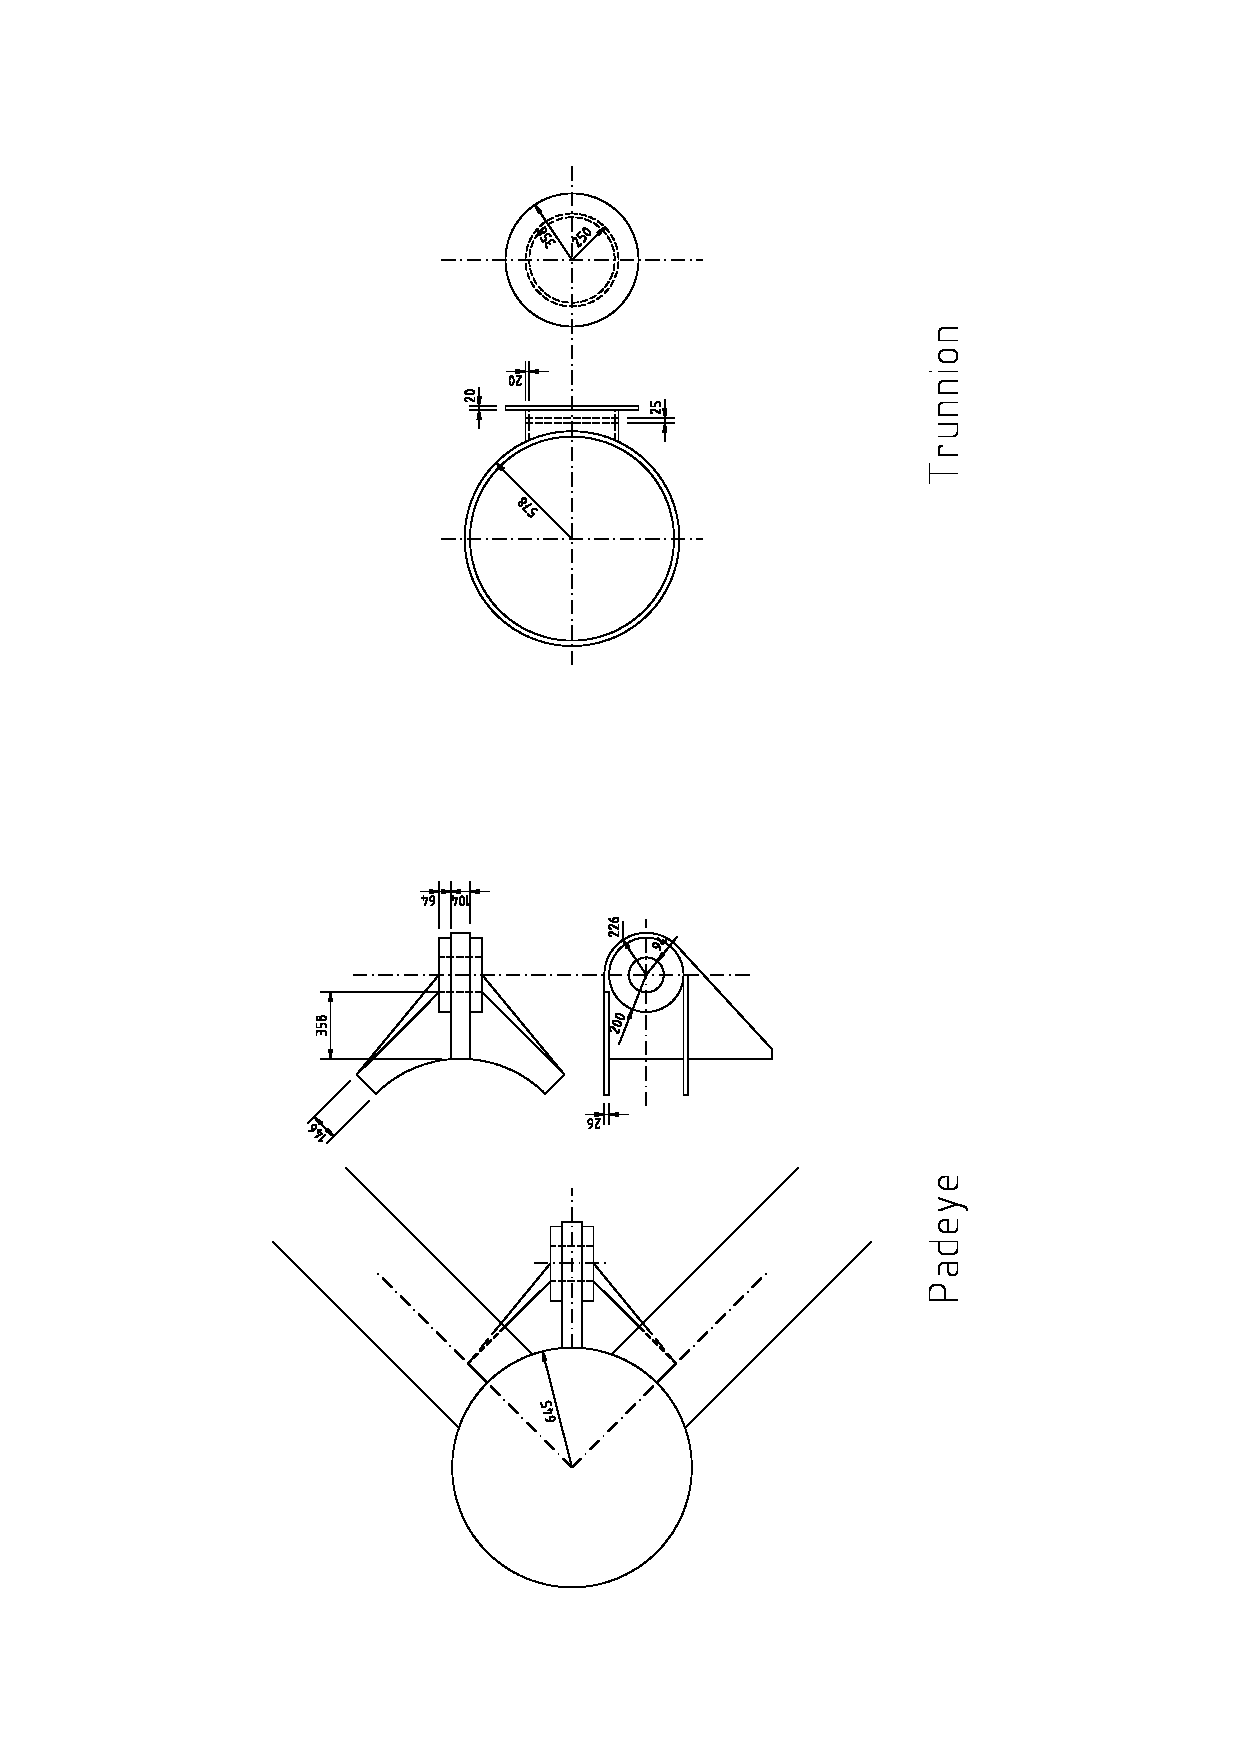
\includepdf[landscape, angle=-90]{dimensions}


\end{document}
